\chapter{Aplicações de Transformações Lineares}
As TL têm contribuições significativas para o campo da AL. \cite{strang2010}, renomado matemático e professor do MIT - Massachusetts Institute of Technology, aborda, por exemplo, o processamento de sinais e imagens para compressão, filtragem, reconstrução e análise de dados, a análise de redes e sistemas dinâmicos da engenharia elétrica e ciência da computação, a geometria e a computação gráfica para manipular objetos em espaços tridimensionais, videogames e modelagem em três dimensões, além de cripto segurança e, mais recentemente, análise de dados em decisões gerenciais e aprendizagem de máquina. \nocite{pitombeira1971}

A seguir, baseando em um estudo desenvolvido na Universidade Federal de Alagoas \cite{sirlandro2017}, apresentamos algumas aplicações das TL na área de engenharia.

\section{Circuitos Elétricos}
Um circuito elétrico é composto por geradores que criam correntes elétricas com magnitudes limitadas pelos resistores posicionados em série ou em paralelo, exemplificado na figura 12. Existem três unidades básicas da física: potencial elétrico $\mathbf{V}$(volts = $\mathbf{V}$), resistência elétrica $\mathbf{R}$(ohms = $\Omega$) e corrente elétrica $\mathbf{I}$(ampères = $\mathbf{A}$), como por exemplo, baterias, que mantêm a diferença de potencial constante entre seus dois terminais.

\begin{figure}[H]
	\centering
	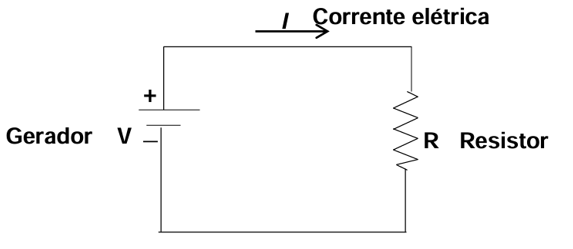
\includegraphics[scale=0.90]{a_fg1.png}
	\caption{Diagrama de circuito elétrico \cite{sirlandro2017}.}
\end{figure}

Para a montagem ou avaliação de um circuito, é necessário descobrir qual a corrente elétrica que passa em cada trecho do circuito e as quedas de potencial. Dependendo do fluxo da corrente elétrica, as intensidades de corrente e as quedas de tensão podem ser positivas ou negativas. Três princípios básicos devem ser considerados:

\begin{itemize}
	\item \textbf{Lei de Ohm:} A diferença de potencial medida através de um resistor é o produto da corrente que passa por ele e a sua resistência, representado por
	
	\centerline{$\mathbf{V} = \mathbf{R} \times \mathbf{I}$},
	onde $\mathbf{V}$ é a tensão, em Volts($\mathbf{V}$, $\mathbf{R}$ é a resistência, em ohm($\Omega$) e $\mathbf{I}$ é a corrente, em ampère($\mathbf{A}$).
	
	\item \textbf{Lei da corrente de Kirchhoff:} Se houver um ponto de ramificação, junção ou nó, a corrente pode se dividir e a soma das correntes que chegam no nó devem ser iguais à soma das correntes que saem do nó, representado por
	
	\centerline{$\mathbf{I} = \mathbf{I}_1 + \mathbf{I}_2$}
	
	\item \textbf{Lei das malhas ou Lei de Voltagem de Kirchhoff:} A soma algébrica das variações no potencial ao longo de qualquer malha fechada deve ser igual a zero. Para exemplificar a aplicação das leis, considera-se o circuito da figura
	
	\begin{figure}[H]
		\centering
		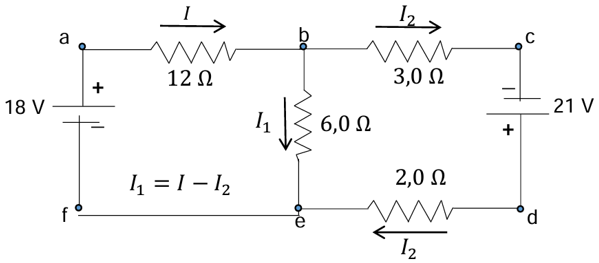
\includegraphics[scale=0.90]{a_fg2.png}
		\caption{Circuito de malha de resistência elétrica \cite{sirlandro2017}.}
	\end{figure}
\end{itemize}

Considerando a lei dos nós no trecho $\overrightarrow{abefa}$, obtemos a equação

\centerline{$18\mathbf{V} - (12\Omega)\mathbf{I} - (6\Omega)\mathbf{I}_1 = 0$}

Aplicando a lei das malhas no trecho $\overrightarrow{abefa}$, obtemos a equação

\centerline{$-(3\Omega)\mathbf{I}_2 + 21\mathbf{V} - (2\Omega)\mathbf{I}_2 + (6\Omega)\mathbf{I}_1 = 0$}

Para determinar as correntes, resolvemos o sistema de equações lineares

\begin{enumerate}
	\item $\mathbf{I} = \mathbf{I}_1 + \mathbf{I}_2$
	\item $18 - 12\mathbf{I} - 6\mathbf{I}_2 = 0$
	\item $21 - 5\mathbf{I}_2 + 6\mathbf{I}_1 = 0$
\end{enumerate}

Dividimos a equação 2 por 6:

\begin{enumerate}
	\item $\mathbf{I} = \mathbf{I}_1 + \mathbf{I}_2$
	\item $3 - 2\mathbf{I} - \mathbf{I}_1 = 0$
	\item $21 - 5\mathbf{I}_2 + 6\mathbf{I}_1 = 0$
\end{enumerate}

Representado em matriz aumentada, temos o sistema consistente

\[
\left[
\begin{array}{ccc|c}
	1 & -1 & -1 & 0\\
	-2 & -1 & 0 & -3\\
	0 & 6 & -5 & 21\\
\end{array}
\right]
\]

Utilizando o método de Gauss-Jordan, podemos adotar a seguinte sequência:
\begin{enumerate}
 
	\item Multiplicar a primeira linha por 2:
	\[
	\begin{bmatrix}
		2 & -2 & -2 & 0 \\
		-2 & -1 & 0 & -3 \\
		0 & 6 & -5 & 21 \\
	\end{bmatrix}
	\]
	
	\item Somar o resultado à linha 2:
	\[
	\begin{bmatrix}
		2 & -2 & -2 & 0 \\
		0 & -3 & -2 & -3 \\
		0 & 6 & -5 & 21 \\
	\end{bmatrix}
	\]
	
	\item Multiplicar a linha 2 por 2:
	\[
	\begin{bmatrix}
		2 & -2 & -2 & 0 \\
		0 & -6 & -4 & -6 \\
		0 & 6 & -5 & 21 \\
	\end{bmatrix}
	\]
	
	\item Somar o resultado à linha 3:
	\[
	\begin{bmatrix}
		2 & -2 & -2 & 0 \\
		0 & -6 & -4 & -6 \\
		0 & 0 & -9 & 15 \\
	\end{bmatrix}
	\]
	
	\item Multiplicar a linha 3 por $-\frac{1}{9}$:
	\[
	\begin{bmatrix}
		2 & -2 & -2 & 0 \\
		0 & -6 & -4 & -6 \\
		0 & 0 & 1 & -\frac{5}{3} \\
	\end{bmatrix}
	\]
	
	\item Multiplicar a linha 3 por 1:
	\[
	\begin{bmatrix}
		2 & -2 & -2 & 0 \\
		0 & -6 & -4 & -6 \\
		0 & 0 & 1 & -\frac{5}{3} \\
	\end{bmatrix}
	\]
	
	\item Somar à linha 1:
	\[
	\begin{bmatrix}
		2 & -2 & -1 & -\frac{5}{3} \\
		0 & -6 & -4 & -6 \\
		0 & 0 & 1 & -\frac{5}{3} \\
	\end{bmatrix}
	\]
	
	\item Multiplicar a linha 3 por 2:
	\[
	\begin{bmatrix}
		2 & -2 & -1 & -\frac{5}{3} \\
		0 & -6 & -4 & -6 \\
		0 & 0 & 2 & -\frac{10}{3} \\
	\end{bmatrix}
	\]
	
	\item Somar à linha 2:
	\[
	\begin{bmatrix}
		2 & -2 & -1 & -\frac{5}{3} \\
		0 & -6 & -2 & -\frac{28}{3} \\
		0 & 0 & 2 & -\frac{10}{3} \\
	\end{bmatrix}
	\]
	
	\item Multiplicar a linha 2 por $-\frac{1}{3}$:
	\[
	\begin{bmatrix}
		2 & -2 & -1 & -\frac{5}{3} \\
		0 & 2 & \frac{2}{3} & \frac{28}{9} \\
		0 & 0 & 2 & -\frac{10}{3} \\
	\end{bmatrix}
	\]
	
	\item Somar à linha 1:
	\[
	\begin{bmatrix}
		2 & 0 & -\frac{2}{3} & \frac{13}{9} \\
		0 & 2 & \frac{2}{3} & \frac{28}{9} \\
		0 & 0 & 2 & -\frac{10}{3} \\
	\end{bmatrix}
	\]
\end{enumerate}

Iara, os passos dão errado para o resultado final...

 
